\scanpage{36}
\figure{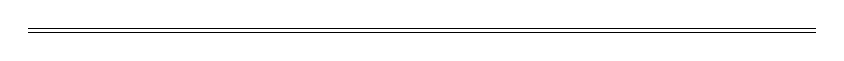
\begin{tikzpicture}\draw (0,0)--(10,0);\draw (0,-.05)--(10,-.05);\end{tikzpicture}}

\textsc{Algèbre.} --- \textit{Définition des classes de Stiefel-Whitney d'un module
quadratique sur un corps de caractéristique différente de 2.}
Note de M. \textbf{\textsc{Antoine Delzant}}, transmise par M. Jean Leray.

Soit $\mathrm A$ un corps de caractéristique différente de 2. On ne considère que
des modules quadratiques $(\mathrm E,\mathrm Q)$ $^{(1)}$, de rang fini sur $\mathrm A$,
et non dégénérés.

On désigne par $\mathrm Q^+$ l'ensemble des classes à isomorphisme près de modules
quadratiques. L'ensemble $\mathrm Q^+$ est muni de deux opérations : l'une, la somme
directe externe, définit sur $\mathrm Q^+$ une structure de monoïde abélien pour laquelle
tous les éléments sont réguliers (théorème de Witt); l'autre, le produit tensoriel,
est commutative, distributive par rapport à la précédente, et admet un élément unité
[la classe du module $(\mathrm A,\mathrm I)$, où $\mathrm I(x)=x^2$].
L'ensemble $\mathrm Q^+$ se plonge donc injectivement dans un anneau $\mathrm Q(\mathrm A)$,
qu'il engendre. L'anneau $\mathrm Q(\mathrm A)$, commutatif avec élément unité, est appelé
l'\textit{anneau des classes de formes quadratiques}. A toute classe $q$ de module
quadratique $(\mathrm E,\mathrm Q)$ on fait correspondre $\varepsilon(q)=rg(\mathrm E)$;
on définit ainsi un homomorphisme d'anneau de $\mathrm Q(\mathrm A)$ dans $\mathbf Z$
appelé l'augmentation.

Soit $\mathrm A_s$ la clôture séparable de $\mathrm A$ et $\mathrm G$ le groupe de Galois
de $\mathrm A_s$ sur $\mathrm A$; on note $\mathrm H^q(\mathrm A,\mathbf Z/2\mathbf Z)$
le $q^{\text{ième}}$ groupe de cohomologie de $\mathrm G$ à valeurs dans
$\mathbf Z/2\mathbf Z$. On note additivement le groupe $\mathrm A^\star$,
groupe multiplicatif de $\mathrm A$, et l'on pose
$\mathrm D(\mathrm A)=\mathrm A^\star/2\mathrm A^\star$.
Le groupe $\mathrm D(\mathrm A)$ s'identifie à
$\mathrm H^1(\mathrm A,\mathbf Z/2\mathbf Z)$.

Soit $a$ un élément de $\mathrm A^\star$; on note $e_a$ sa classe dans
$\mathrm D(\mathrm A)$, et $\varphi_a$ la classe du module quadratique
$[\mathrm A,\mathrm Q;\ \mathrm Q(x)=ax^2]$.
L'élément $\varphi_a$ ne dépend que de $a$ modulo $2\mathrm A^\star$;
on peut donc définir un homomorphisme de $\mathrm D(\mathrm A)$ dans le groupe
multiplicatif $\mathrm Q(\mathrm A)^\star$ des éléments inversibles de $\mathrm Q(\mathrm A)$.
D'où un homomorphisme d'anneaux :
\[
\varphi:\quad\mathbf Z(\mathrm D)\to\mathrm Q(\mathrm A),
\]
où $\mathbf Z(\mathrm D)$ est l'algèbre de $\mathrm D(\mathrm A)$ sur $\mathbf Z$,
munie de la filtration définie par les puissances de l'idéal d'augmentation.

\textsc{Proposition.} --- \textit{L'application $\varphi$ est surjective; elle est
compatible avec les augmentations; le noyau de $\varphi$ est l'idéal engendré
par les éléments $e_a+e_b-e_{a'}-e_{b'}$, tels que
$\varphi_a+\varphi_b=\varphi_{a'}+\varphi_{b'}$.}

Le cup-produit définit une application de $\mathrm D(\mathrm A)\times\mathrm D(\mathrm A)$
dans $\mathrm H^2(\mathrm A,\mathbf Z/2\mathbf Z)$ notée $(e_a,e_b)\to a.b$.
Si l'on identifie $\mathrm H^2(\mathrm A,\mathbf Z/2\mathbf Z)$ au sous-groupe
du groupe de Brauer de $\mathrm A$ formé des $x$ tels que $2x=0$, l'élément $a.b$
\mspage{35}
